\chapter{Related Work}

%% Add more to introduce topics in this chapter?

\section{Dormitory Energy Competitions}
\label{sec:dorm-energy-competitions}

Energy competitions in residence halls have become a popular event at colleges and universities. The residence halls compete to see which building will use the least energy over a period of time. Some competitions pull in other aspects of environmental sustainability, including reducing water usage, reduced waste production, etc. The competitions tap into both the residents competitive urges, and the interest in environmental issues. However, unlike a home environment, the residents do not financially benefit from any reduction in electricity use resulting from their behavior changes, since residence hall fees are flat-rate and do not change based on energy usage. This leads to residents being completely unaware of their energy usage, since they lack even a monthly bill as feedback.

The most basic type of energy competition website displays energy data which is updated manually on a periodic basis (such as weekly). The Wellesley College Green Cup \cite{wellesley-green-cup} is an example of this type of competition.

Other schools have more complicated and interactive competition websites, such as the early adopter Oberlin College. Petersen et al.\ describe their experiences deploying a realtime feedback system in an Oberlin College dorm energy competition in 2005 \cite{petersen-dorm-energy-reduction}. 22 dormitories were in competition over a 2 week period, with 2 dorms having feedback updates every 20 seconds, and the other 20 getting updates every week. The realtime dorms also recorded electricity usage for each of the three floors, but only displayed the data from two of the floors, leaving the third as a control. Web pages were used to provide feedback to students, since they all have computers and Internet access in their rooms. They found a 32\% reduction in electricity use across all dormitories, with the 2 realtime feedback dorms reducing usage the most. Freshman dorms were among the highest electricity reducers, while upperclassman dormitories were quite low (average 2\% reduction). During a 2 week post-competition period, the average electricity usage was similar to consumption levels during the competition. However, the weather was warmer and there was more sunlight during the post-competition period, so it is unclear if the reduction was competition-related.

In terms of participation, Petersen et al.\ found 46\% of residents looked at the competition website at least once (based on web server logs mapping IP addresses to residence halls). 23\% of dormitory residents filled out the online post-competition survey. Survey respondents indicated that some behaviors, such as turning off hallway lights at night and unplugging vending machines were not sustainable outside the competition period.


\section{Energy Feedback}
\label{sec:energy-feedback}

To reduce energy use, people must know how much energy they are is using. Feedback systems display the consumption of a resource (such as electricity) to the user, usually in real time. Darby provides a detailed survey of studies on electricity feedback systems from the past 3 decades \cite{darby-review-2006}. The survey of 20 studies finds that, on average, the introduction of a direct (real-time) feedback system leads to reductions of energy usage ranging from 5-15\%. Feedback systems providing historical data (such as those provided with billing statements) are not as effective (0-10\% reductions), but can be useful for assessing the impact of efficiency measures such as improved insulation or a more energy efficient appliance, since those savings accumulate over time.

Darby found that ``consumption in identical homes, even those designed to be low-energy dwellings, can easily differ by a factor of two or more depending on the behaviour of the inhabitants.'' This finding demonstrates the significant potential to curb energy usage through changes in individual's behavior.

Another survey of energy feedback was conducted Faruqui et al., looking at 12 utility pilot programs that installed in-home displays with near-realtime feedback \cite{Faruqui09}. They found that customers that actively used the display averaged a 7\% reduction in energy usage, while those pilot programs that included pre-paid electrical services reduced their energy usage by 14\%. The sustainability of the energy reduction is unclear based on the pilot studies since they were of limited length. The authors believe it is unknown whether the residents of homes with displays will acclimate to the display and cease to use it to reduce their energy usage.

Darby also points out that while feedback is critical for energy conservation behaviors, feedback alone is not always enough \cite{darby-2000-making-it-obvious}. Other factors that lead to higher rates of energy conservation include contact with an advisor when needed, and training and social infrastructure.

\begin{figure}[htbp]
	\centering
		\includegraphics[scale=0.59]{current-energy-website}
		\caption{View of LBNL's Current Energy Web Site on December 15, 2004}
		\label{fig:current-energy-website}
\end{figure}

During California's energy crisis in 2000 and 2001, Lawrence Berkeley National Laboratory created a web site that graphed data from utility organizations \cite{Bartholomew2008Current-Energy}. The graphs showed consumer demand for electricity (actual and forecast), and the utilities' generation capacity (see \autoref{fig:current-energy-website} for an example graph). Darby reports anecdotal evidence that people viewing the graphs changed their electricity usage based on the data \cite{darby-review-2006}.

\fxnote{Add Ecotricity ref here?}

There is also evidence that just the knowledge that one is being monitored can cause one to consume fewer resources. A group of researchers simulating a mission to Mars or the Moon in the Canadian Arctic for four months tracked the crew members' water usage \cite{Bamsey2008FMARS}. Water usage was monitored via automated meters during the entire mission, but during certain multi-day study periods, crew members were also required to manually log their water usage at the point of use. The authors found that water usage was 10\% less during these study periods. The reduced water usage could be due to the knowledge that the usage was being examined more closely, or perhaps the extra effort required to manually record their water usage led to crew members reducing non-essential water use (see \autoref{sec:ecoisland} for another possible benefit to manual data collection).

\begin{figure}[htbp]
	\centering
		\subfigure[Device itself]{\label{fig:thighmaster-device}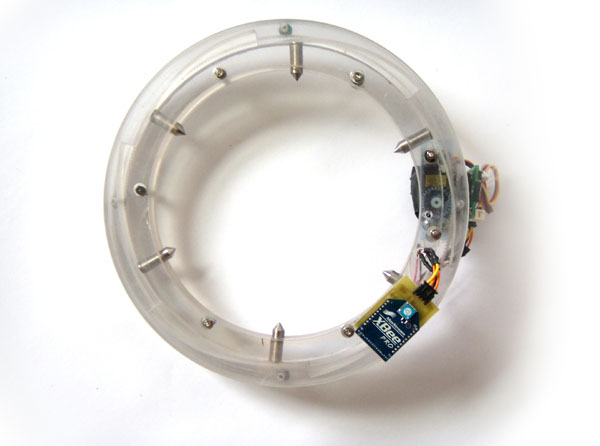
\includegraphics[height=2.5in]{thighmaster-alone}}
		\subfigure[As worn on leg]{\label{fig:thighmaster-leg}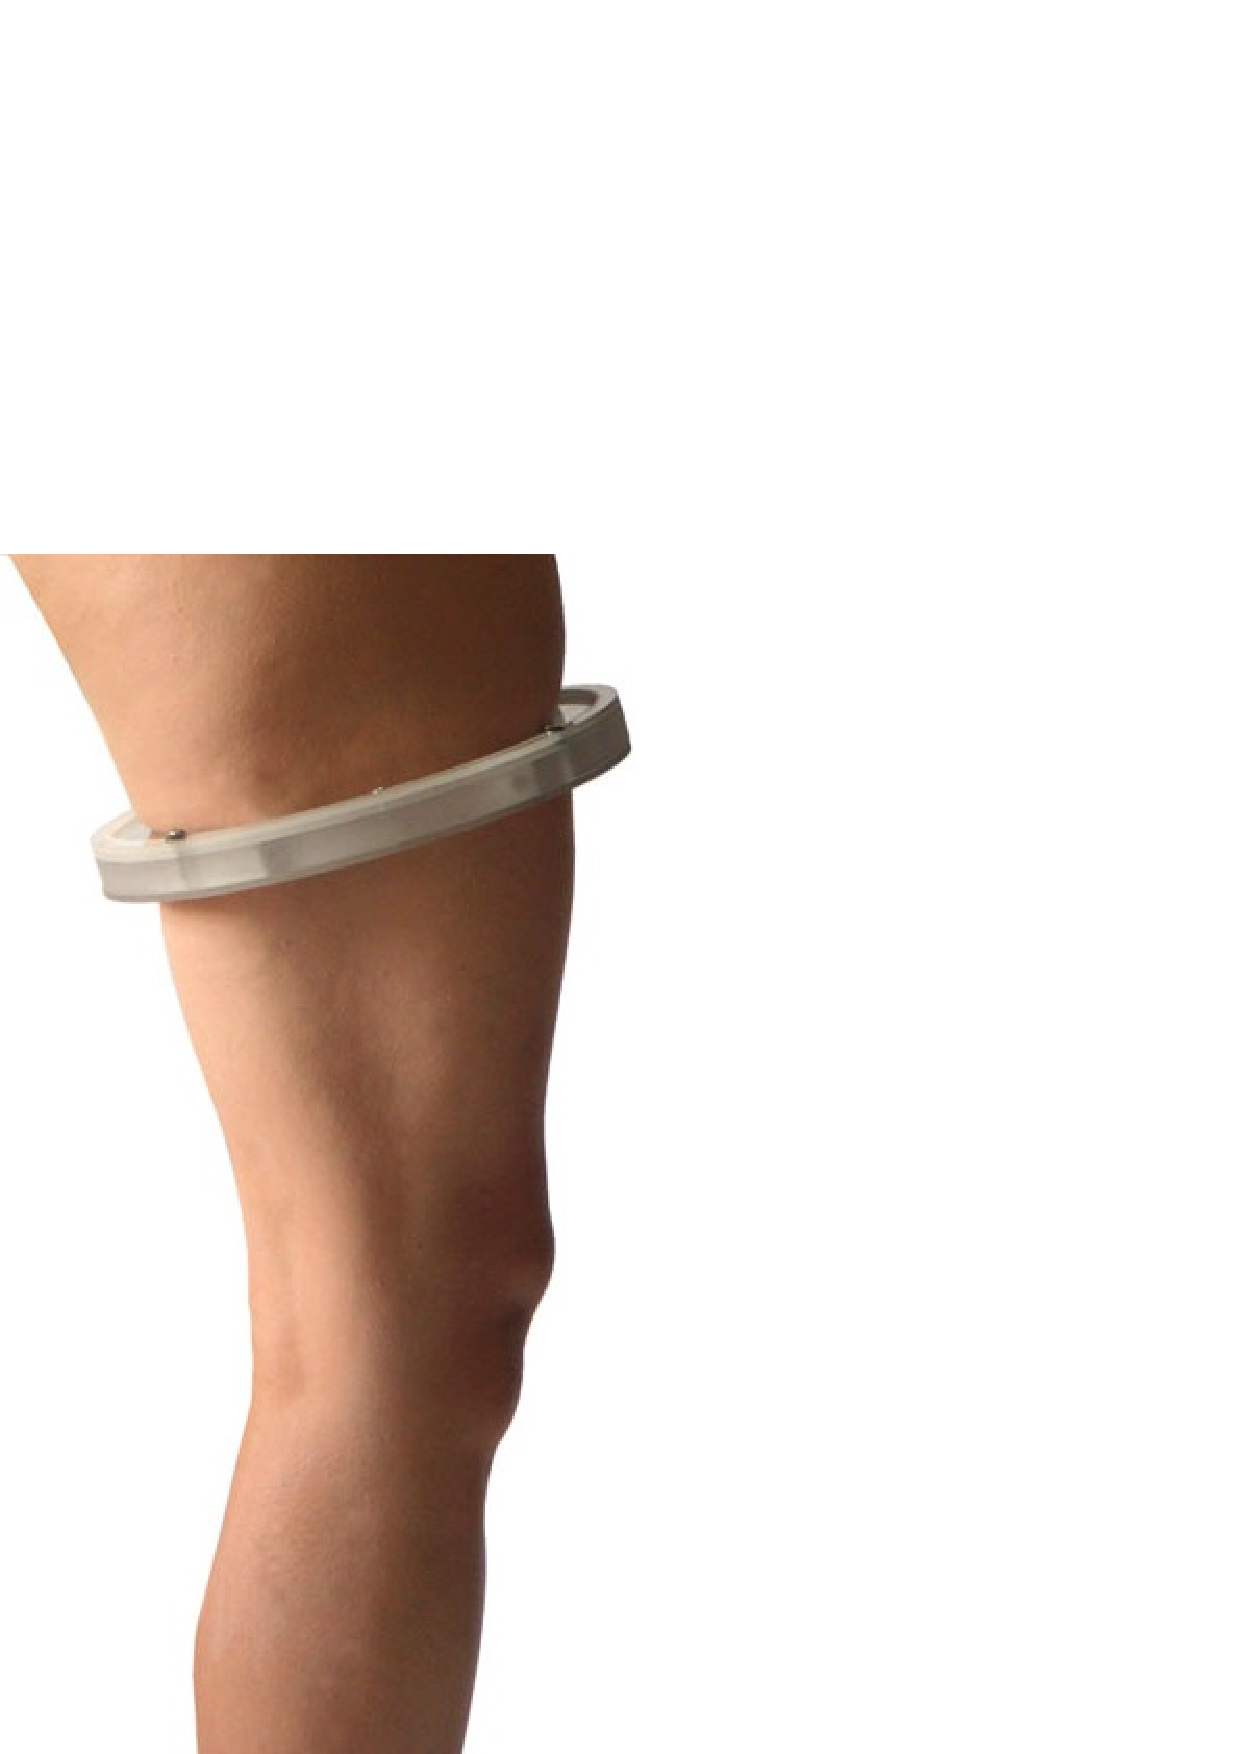
\includegraphics[height=2.5in]{thighmaster-leg}}
		\caption{Thighmaster energy feedback mortification device}
		\label{fig:thighmaster}
\end{figure}

R\"{u}st has implemented an extreme energy feedback system called the Thighmaster \cite{Rust2008Thighmaster-web}. Inspired by the cilice (a small metal garter with inward facing spikes) worn by some members of the Catholic Opus Dei organization as part of a practice of mortification, the Thighmaster is a ``techno-garter'' that pokes the wearer with spikes when their actions are not environmentally responsible (as defined by R\"{u}st), see \autoref{fig:thighmaster} for a depiction of the device. Specifically, the Thighmaster communicates wirelessly with electricity usage sensors and a human speech sensor that monitors whether the user speaks with their plants. While more of a demonstration, the Thighmaster shows the complex emotions involved in people's reactions to climate change. It goes without saying that being pierced by spikes is unlikely to be a viable energy feedback mechanism for most users.


\section{Related Systems}
\label{sec:related-systems}

In this section we examine other systems that have been designed to help users become more aware of their environmental impact, or make environmentally-positive behavior changes.

In a position paper, Sutaria and Deshmukh describe using networks of ad hoc sensors to monitor both electricity usage and miles driven by automobile, while providing real-time feedback to the user \cite{sutaria-2008}. The system described would compare the household's energy usage with others in similar situations. They envision smart energy meters that can also provide suggestions on how users can reduce their energy usage. They also mention the possibility of integrating personal carbon trading (a sort of carbon cap-and-trade system for individuals) into the system. The system described by Sutaria and Deshmukh appears to be hypothetical at this point.

\subsection{StepGreen}
\label{sec:stepgreen}

StepGreen is a web application designed to encourage people to undertake environmentally responsible actions \cite{step-green-website}. Mankoff et al.\ have written about the rationale for the system and description of the design, presumably written before the site was active \cite{Mankoff2007Leveraging-Soci} \fxnote{Should update with more recent StepGreen paper(s)}. The paper introduces the fact that, in the U.S., half of a person's energy consumption is their control. Therefore, by modifying their behaviors, Americans can affect up to half their \COtwo emissions. StepGreen (also known as Footsteps, possibly an earlier name for the system) is designed to leverage online social networks to motivate personal change, by providing suggestions for improvement.

\begin{figure}[htbp]
	\centering
		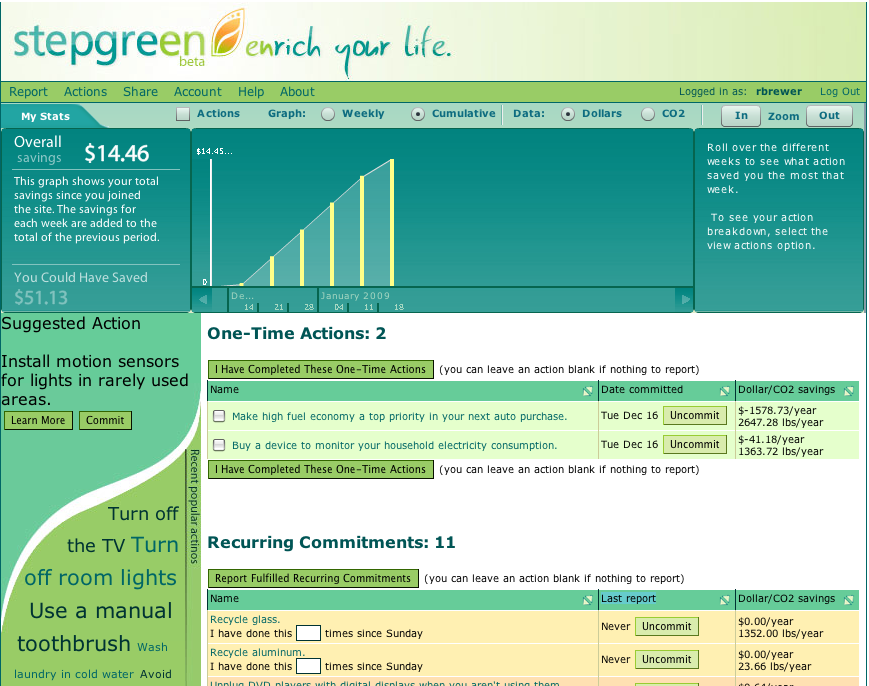
\includegraphics[width=\textwidth]{stepgreen-bitmap}
		\caption{Example page from StepGreen website}
		\label{fig:stepgreen-website}
\end{figure}

The StepGreen system is currently open to the public. \autoref{fig:stepgreen-website} shows an example of the default page shown when a user logs in. Users create an account on StepGreen, and then are presented with a list of actions with positive environmental consequences (mostly reduced GHG emissions). Example actions are ``Turn off the lights when you exit the house in the morning for the day'', ``Take the stairs at work'', and ``Set your home computer to automatically hibernate/sleep after a short period of inactivity''. Each action is associated with its cost savings and reduction in \COtwo emissions. Users can get more information about the action and how the savings were calculated. For each action, users can indicate whether they are already performing that action, whether they commit to undertaking that action, or whether the action is not applicable to them. Users can create new actions to be added to the list, but since the new actions have not been analyzed by the site maintainers, the financial and \COtwo savings are listed as unknown.

Once users have selected actions that they are either already performing or commit to performing, they can track them on the Reporting page. For one time actions, such as replacing an incandescent light bulb with a compact florescent bulb, users simply check off when they are completed. For recurring actions, users must indicate how many times they have performed the action since their last report in order for the system to track the activities. Based on the user's self-reporting, StepGreen calculates the amount of money saved, pounds of \COtwo saved (i.e., reduced), and missed pounds of \COtwo saved, and provides a historical graph of these values.

StepGreen also provides links to social networking sites. They provide a linked Facebook application, a MySpace profile widget, and a connection to Twitter. Each of these links provides a way to inform the user's social network about what actions the user is undertaking. This feature can serve to recruit other people to use StepGreen, provide comparisons on financial and environmental savings among peers, and encourage users to keep to their StepGreen commitments. 

StepGreen provides a useful platform for research on convincing users to change their behavior to reduce their carbon footprint. For example, a virtual polar bear was implemented to motivate users to reduce their carbon footprint (see \autoref{sec:virtual-polar-bear}). Notes on the StepGreen research website \cite{stepgreen-research-website} indicate that there are plans to support the input of sensor data from the UbiGreen transportation sensing project that they are a part of \cite{ubigreen-website}.

In its current state, StepGreen would be challenging to keep up to date due to the reliance on manual data input. Due to the limitations of manual reporting, StepGreen may report missed savings that are not accurate, annoying users. For example, recycling glass is an action that is listed as having substantial carbon savings. However, if one chooses to drink water from a mug instead of purchasing a beverage and later recycling the glass container, clearly the carbon savings are greater from using the mug, but StepGreen will count the lack of recycling as missed savings.

\subsection{Personal Kyoto}
\label{sec:personal-kyoto}

Personal Kyoto is a web service that tracks the electricity usage of users in the New York area, and compares it to a ``Personal Kyoto Goal'' for the user \cite{Personal-Kyoto-website}. The Personal Kyoto Goal represents the limit of electricity usage that would apply to the user if the Kyoto Protocol (which the USA is not a party to) were administered on an individual basis rather than on a national basis.

The user's electricity usage is retrieved from the local utility's web site (Con Edison) using the user's account number. In addition to the monthly usage (which can vary substantially due to circumstances and the seasons), a 12 month rolling average is computed to remove the seasonal effects. The Personal Kyoto Goal is defined as 75\% of the first point of the monthly rolling average when the user signed up with the web site. \autoref{fig:personal-kyoto} shows an example graph with monthly averages and a personal Kyoto goal.

\begin{figure}[htbp]
	\centering
		\includegraphics[width=\textwidth]{personal-kyoto}
		\caption{Example graph of electricity usage from Personal Kyoto}
		\label{fig:personal-kyoto}
\end{figure}

Personal Kyoto is a cleverly designed system in that it uses the user's real data, but avoids manual data entry by scraping the data from the utility web site. It also gives the user a specific goal for reducing electricity use that has a real justification and ties into the environmental ``gravitas'' of the Kyoto Protocol.

\subsection{EcoIsland}
\label{sec:ecoisland}

Takayama and Lehdonvirta have constructed a system they call EcoIsland, which attempts to ``motivate behaviour changes that reduce CO2 emissions'' using a background game-like activity, with a centrally installed display in the home \cite{takayama-2008}. \autoref{fig:ecoisland} shows an example of the user interface. Each family member has an avatar on the virtual island, and they set a family \COtwo emissions target. The family's emissions are tracked via sensors and self-reporting. If the emissions exceed the chosen target level, the water level on the island rises, and if the water level continues to rise it will eventually end the game.

\begin{figure}[htb]
	\centering
		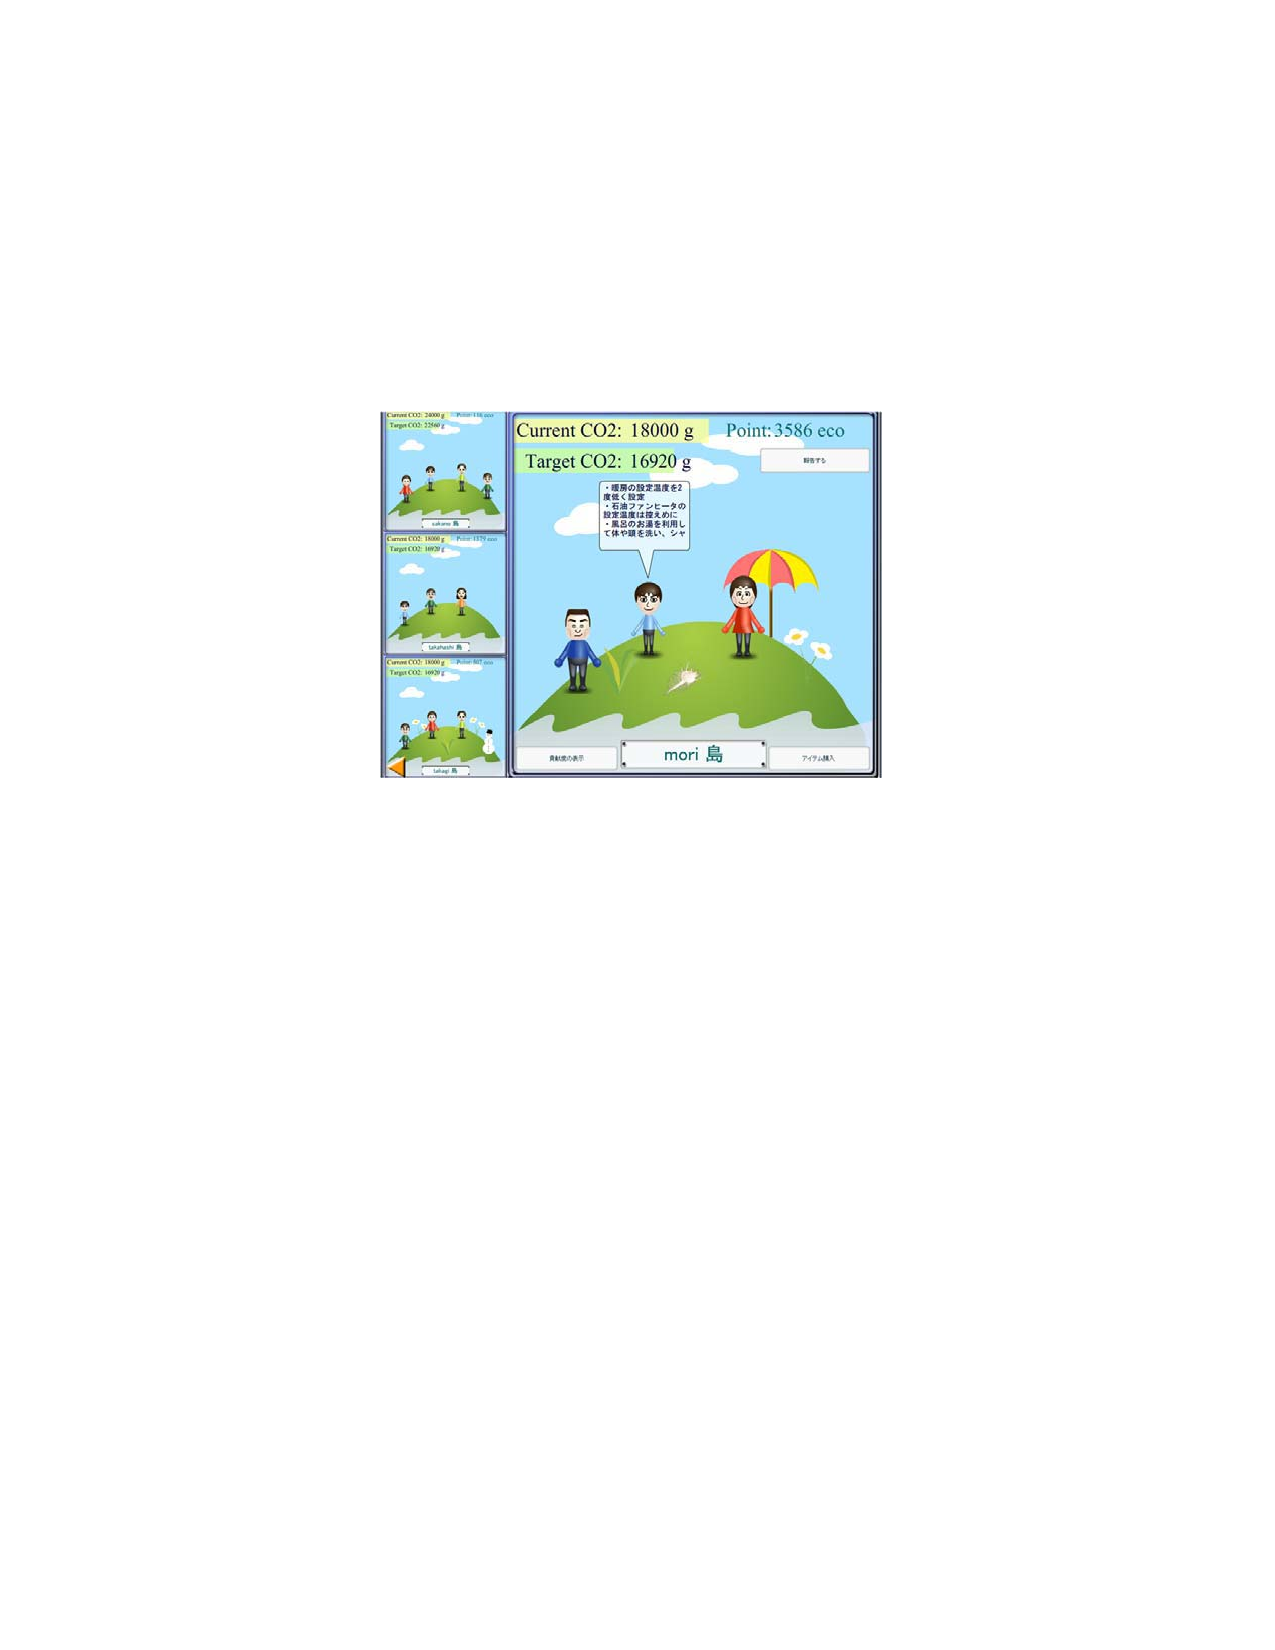
\includegraphics[width=0.8\textwidth]{ecoisland}
		\caption{Example EcoIsland display, with family avatars}
		\label{fig:ecoisland}
\end{figure}

Participants mobile phones have a list of suggested actions to reduce emissions, and they can self-report their actions using the phone. Participants can see the islands of other participants and they receive a periodic allowance in a virtual currency. The participants can use the virtual currency to buy decorations for their island, or to purchase carbon credits from other users. Participants with low emissions, therefore, can decorate their island, while those with high emissions have to spend their money on carbon credits. EcoIsland provides a metaphor for the users' emissions and makes them aware of the consequences of their actions.

The sensor portion of the system was not yet implemented at the time the authors conducted their study. The authors performed a four week pilot study of EcoIsland with 20 people in six families. During the first week, the baseline electricity usage of each participant's air conditioning system was monitored using a plug load meter (for more information on this type of meter, see \autoref{sec:plug-load-meters}). During the second week, one participant from each household was asked to use the system, while in the third week all members were asked to use it. In the fourth week, the carbon trading system was introduced to participants. At the conclusion of the study, the participants were surveyed and 17 of 20 participants said ``they were more conscious of environmental issues after the experiment than before.'' However, users indicated that they were motivated by game issues (such as saving the sinking island and buying in-game decorations) rather than saving the environment. Few of the participants used the carbon trading system because their targets were easy enough to achieve without trading. Air conditioner usage in participant homes showed no correlation with game outcome, but the authors believe that the short study may have affected that outcome. The study was conducted in winter, which might seem like an inappropriate time to measure air conditioner use. However, in Japan, many air conditioning units also function as heaters, so it may be this type of air conditioner usage that the authors are referring to. One interesting result is that participants noted that manual reporting contributed to their motivation, so replacing the reporting with sensors could reduce user's motivation to change.

\subsection{Google PowerMeter}
\label{sec:google-powermeter}

Utilities are starting to install `smart meters' (also called AMI for Advanced Metering Infrastructure) on homes as part of an overall push towards the `smart grid'. However, these smart meters are often thought about from the utility's perspective: eliminating manual meter reading, enabling time-of-day electricity pricing, and monitoring power reliability. While there are many benefits for the utility, frequently updated power data from the meter could be very useful if provided directly to the people being metered, as discussed in \autoref{sec:energy-feedback}.

Google PowerMeter is a web application developed to make smart meter data available to the end users living in smart metered homes \cite{Google-PowerMeter}. Google partners with utilities that have rolled out smart meters, and collects the power data from the utility. PowerMeter also works with the TED 5000 home energy meter that can be installed by end-users without interaction with the utility (see \autoref{sec:whole-home-meters}). The data is recorded at 15 minute intervals, and presented in a variety of graphs that show daily usage and home base load levels. \autoref{fig:google-powermeter} shows an example display for a home in \Hawaii. The primary interface for PowerMeter is a web gadget that is installed on the user's iGoogle home page. PowerMeter allows users to share their data with others, and has added an API to allow users to get access to their raw data.

\begin{figure}[htbp]
	\centering
		\includegraphics[width=\textwidth]{google-powermeter}
		\caption{Google PowerMeter data for a home in \Hawaii}
		\label{fig:google-powermeter}
\end{figure}

%\subsection{Microsoft Hohm}

\subsection{Virtual Polar Bear}
\label{sec:virtual-polar-bear}

Dillahunt et al.\ (who are involved with the StepGreen project) have built a system providing a virtual polar bear that is affected by the user's environmental choices as a means to motivate users to reduce their carbon footprint \cite{dillahunt-virtual-polar-bear-2008}. They note that there are strong emotional bonds between humans and animals, which may help to encourage environmentally-responsible behavior. The authors performed a one week study, with subjects divided into two groups: an attachment group and a control group. The attachment group read a story about climate change impacting polar bear habitats, and were asked to name their virtual polar bear. As participants make or decline commitments to environmentally responsible actions, the ice under polar bear either grows or shrinks (see \autoref{fig:virtual-polar-bear} for images of the polar bear). The study had 20 subjects (10 for each group), all of whom were surveyed before and after to test for levels of empathy and environmental concern. The subjects in the attachment group had more fulfilled environmental commitments, which was a statistically significant difference. The attachment subjects also had a greater level of environmental concern after interacting with the polar bear. The authors were unsure whether effects would be sustained in a longer study. They are now working on bringing the system to a mobile platform and creating a polar bear application for Facebook and MySpace.

\begin{figure}[htbp]
	\centering
		\includegraphics{virtual-polar-bear}
		\caption{Example images of virtual polar bear with lots of ice and with little ice}
		\label{fig:virtual-polar-bear}
\end{figure}

\subsection{iamgreen}
\label{sec:iamgreen}

iamgreen is an application for the Facebook social networking platform that provides an online gathering place for environmentally conscious users \cite{iamgreen-website}. iamgreen provides all of the standard components of Facebook: a newsfeed of events from members, status updates, news articles, etc. The application provides a list of environmentally responsible statements called ``leaves'', such as ``Most of my lightbulbs are compact fluorescents'', ``I recycle, even when it is not convenient'', and ``When I drive, it's over 40mpg baby'' (see \autoref{fig:iamgreen} for an example of the leaf selection page). For each statement, users can indicate if they engage in that behavior, they aspire to that behavior, they wish to hide the statement (removing it from the list of choices), or they want to recommend it to a friend. Users can then display the number of leaves they have committed to in their Facebook profiles. Users can also contribute new leaves, which will be displayed as options to other iamgreen users.

\begin{figure}[htbp]
	\centering
		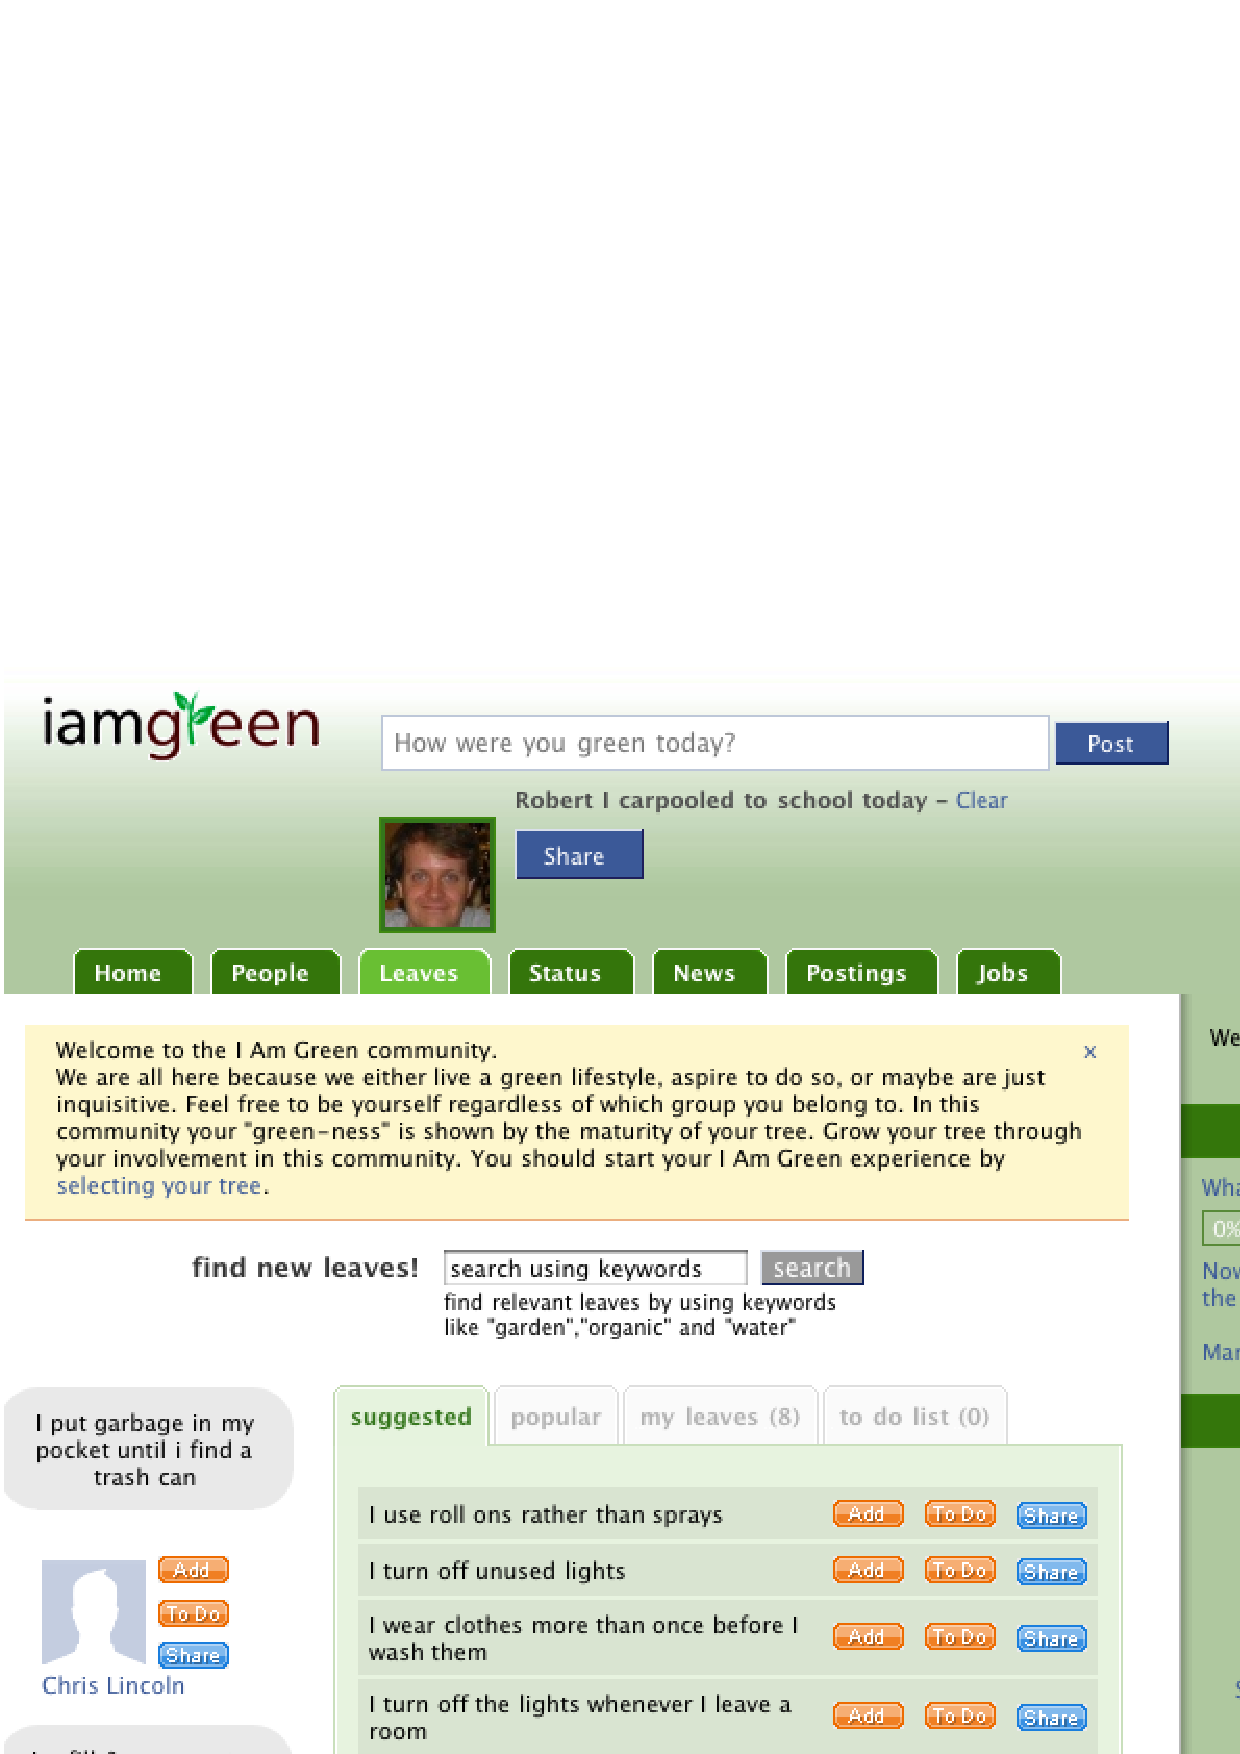
\includegraphics[width=0.8\textwidth]{iamgreen}
		\caption{Leaf selection page of iamgreen Facebook application}
		\label{fig:iamgreen}
\end{figure}

While the leaves concept is a simple way to encourage users to make more environmentally positive choices, it suffers from some obvious deficiencies. First, leaves, for the most part, have the same value (though apparently some actions, such as not owning a car, are worth more than one leaf). The leaf system also lacks any quantitative feedback other than the number of leaves, so the user is not provided with real insight into their environmental footprint. Like any system based on manual reporting, users have to spend time reporting any changes to their action list. Without quantitative feedback, it seems likely that many users will make some selection of leaves and then revisit them infrequently or never again.


\section{Motivation}

De Young investigated the motives behind individual's environmentally responsible behaviors (ERBs) through a series of surveys \cite{Young:2000fv}. Traditionally, the motives invoked by researchers attempting to promote ERB were constrained to material incentives or disincentives and altruistic reasons. The problem with incentives is that they ``needed constant reintroduction to remain effective and they proved to be less reliable than we had hoped''. Incentives can initiate ERB, but people's behavior changes back when the incentives end, and even continuing incentives can have low reliability.

De Young also describes some of the pitfalls that can be encountered in motivating ERB, such as psychological reactance, where people do the opposite of the ERB they are being asked to undertake. Even those initiating the behavior changes can be negatively impacted. De Young describes some initiators experiencing feelings of contempt for those whose behavior they are trying to change, and also contempt for themselves.

Self-interest is generally considered the cause of environmental problems: ``focusing solely on short-term individual or familial gain to the exclusion of long-term societal or environmental benefits''. De Young, however, suggests that self-interest can be a solution to environmental problems. He distinguishes self-interest from selfishness: self-interest meaning each individual is responsible for getting their own needs met. De Young believes that intrinsic satisfaction is a better way to motivate ERB, as people find that ``certain patterns of behavior are worth engaging in because of the personal, internal contentment that engaging in these behaviors provides.''

Based on 9 different studies of ERB across different populations and environmental focuses, the author found 3 intrinsic satisfactions:
\begin{enumerate}
	\item ``satisfaction derived from striving for behavioral competence''
	\item ``frugal, thoughtful consumption''
	\item ``participation in maintaining a community''
\end{enumerate}

Competence involves the enjoyment in completing tasks and solving problems. Frugality is enjoyment from the ``careful stewardship of finite resources''. Participation is the enjoyment from participating in community activities such as sharing news and collaborating with others toward a shared goal.

While attitudes and norms can lead to behavior change, people also need tools and guidance to realize this change. As De Young puts it, ``without considering these variables, we make the error of assuming that once people know what they should do and why they should do it, they will automatically know how to proceed.'' In the particular case of competence as a motivator, it is important to provide people with the opportunity to utilize their competence or they will grow frustrated. He suggests that motivating through competence be accomplished by providing an environment where information on procedures is available and new behaviors can be tried out in a supportive environment.

Darby's survey of electricity feedback programs found similar results on motivations \cite{darby-review-2006}. She found that energy conservation efforts stopped when incentives were removed. When trying to get people to change their behavior, she found that behavior changes formed over a 3 month period is more likely to persist than changes made over shorter periods. She also found that internal motivation is most important for continued conservation efforts.

%In a position paper, Khan and Canny suggest that the technique of social marketing would be helpful in persuading users to make environmentally beneficial changes \cite{Khan2008-social-marketing}. Social marketing is the idea of applying the principles of consumer product marketing to encourage social change. The principles they describe are: emphasis on the benefits of new behavior while minimizing the cost, consumers are strongly influenced by knowing what behaviors others are undertaking. They suggest that target audiences be broken into different market segments, and each segment should receive messages appropriate to that segment. For example, in discussing the iamgreen application (see \autoref{sec:iamgreen}) where users commit to positive environmental actions suggested by others, the authors suggest using collaborative filtering (the technique used by online merchants to suggest other products similar to the one being viewed) to suggest the environmental actions presented to the user rather than just overall popularity of the actions.

\section{Fostering Sustainable Behavior}
\label{sec:fostering-behavior}

A variety of methods have been employed in an attempt to get people to change their behavior to be environmentally sustainable; McKenzie-Mohr provides a good summary of the area in his online book \cite{McKenzie-Mohr2009}. One of the most common techniques is the information-based campaign, which relies on providing information to the public through advertisements and documents like pamphlets and brochures. One type of information campaign attempts to shape peoples' attitudes towards an environmental, in the hope that those new attitudes will lead to more sustainable behavior. Unfortunately, these campaigns are usually unsuccessful. For example, Geller performed an investigation of the impact of three hour workshops on energy conservation that included a survey before and after the workshop \cite{Geller81}. The results of the survey indicated that the workshop had increased the energy literacy of the attendees and they indicated a willingness to implement energy conservation in their homes. However, followup visits with a selected group of 40 of the attendees found that very few had actually taken action (insulating their water heater or installing low-flow showerheads that had been given out during the workshops).

The other type of information-based campaign is based on financial incentives. In energy, this would include a utility advertising the rapid return on investment from a solar hot water heater, or promotion of rebates for more efficient appliances. This approach is also problematic, since it assumes that people are purely rational when making financial decisions, which they are not. For example, in 1983 California utilities were spending ``200 million dollars annually to promote energy conservation'' but with very limited success \cite{Costanzo86}.

To avoid the problems with information-based campaigns, McKenzie-Mohr has developed a process he calls Community-Based Social Marketing (CBSM) \cite{McKenzie-Mohr2009}. The process consists of several steps:

\begin{enumerate}
	\item identifying barriers to the desired behavior, and the benefits of the desired behavior to the individual
	\item developing a strategy to overcome the barriers using behavior change tools
	\item piloting the campaign on a small portion of the intended community, and making changes as needed
	\item evaluating the effectiveness of the campaign on fostering the desired behavior
\end{enumerate}

We focus here on the behavior change tools, which are critical to actually getting people to change their behavior: commitments, goals, and norms.

\subsection{Commitments}

Asking an individual to make a commitment has been shown to be an effective tool in changing behavior. In particular, an initial small, innocuous commitment can lead later to a larger commitment. For example, Freedman and Fraser conducted experiments in which subjects were asked to perform a small task (such as signing a petition to keep California beautiful) and then later asked to perform a more onerous task (such as placing a large billboard on their lawn that said ``Keep California Beautiful'') \cite{Freedman66}. They found that subjects that committed to the small task were much more likely to agree to the second task. The authors call this the ``foot-in-the-door'' technique. One of the reasons this technique is believed to work is the desire by individuals for self-consistency.

Making commitments public can increase their effectiveness. Pallak et al.\ studied residents that were asked to make a commitment to conserve electricity and natural gas \cite{Pallak80}. Some homes were asked to make a private commitment, while others were asked if their commitment could be publicized, though they were never actually published. Those that made commitments that they thought were public conserved more energy than the private committers, even one year later and after they were told that their names were not actually going to be publicized.

\subsection{Goals}

Goals can be thought of as commitments that can be objectively measured, which makes for a good pairing with feedback (see \autoref{sec:energy-feedback}). Becker investigated goal setting along with feedback of home electricity use \cite{Becker78}. Half of the subjects were given a goal of reducing electricity use by 20\% during the summer, the other half were given a goal of 2\%. The subjects given the higher goal conserved between 13\%--15\%, while the group with the smaller goal did no better than a control group. Houwelingen and van Raaij investigated use of natural gas in homes and compared daily feedback with monthly feedback and self reporting, with all groups having a conservation goal of 10\% \cite{Houwelingen89}. The group with daily feedback reduced their energy use by 12.3\%, and some reduction continued in the year after the feedback device was removed from their home.

\subsection{Norms}

Social norms are one way in which people's behavior is influenced by the behavior of others. Cialdini et al.\ make the distinction between descriptive norms (the way things are) and injunctive norms (the way things ought to be) \cite{Cialdini90}. In a series of experiments on littering, they found that subjects that the behavior of confederates of the researchers significantly changed the subjects' behavior. For example, subjects that viewed a confederate littering were more likely to litter a handbill that had been placed on their car. Also, subjects that viewed a confederate littering into a clean environment were less likely to litter than those that observed littering into an environment that already contained a lot of litter.

One problem with descriptive norms is that they can lead to `boomerang effects' where the norm has the effect of decreasing the desired behavior. Schultz et al.\ investigated this issue in the context of home energy conservation \cite{Schultz2007SocialNorms}. 290 homes were divided into two groups: one that would receive a written descriptive norm regarding their energy usage, and one that would receive the descriptive norm plus an injunctive norm. The descriptive norm showed subjects whether they were above or below the average energy usage in their neighborhood. The injunctive norm was simply a frowning or smiling emoticon based on whether the subject home was using more or less than the average consumption respectively. They found that homes that only received the descriptive norm led to energy conservation in homes above the average, but led to increased energy usage in homes below the average (the boomerang effect). However, those homes that also received the injunctive emoticon did not have a boomerang effect. Clearly injunctive norms are an important addition to any attempt to use comparative data to foster energy conservation.

Cultural norms can strongly influence what behaviors are non-negotiable. Strengers performed an ethnographic study of 10 households participating in a smart metering trial to examine how their comfort and cleanliness norms affected their energy savings \cite{strengers-comfort-norms-2008}. Participants were provided with metering devices that displayed electricity and water usage, and greenhouse gas emissions in real time. The author was attempting to use feedback to change the participants societal norms for comfort and cleanliness. For example, until relatively recently, bathing weekly was the norm, but now bathing daily is considered normal behavior. Like many people, the participants did not understand the connection between the consumption data and their practices. Participants tended to increase conservation by changing technology (such as using compact florescent lamps (CFLs) instead of incandescent light bulbs), or by minor behavioral changes like ``taking shorter showers, doing full loads of laundry''.

Strengers states that people act the way they do (in matters of cleanliness and comfort) because ``they believe society expects them to'' and because many companies and organizations have a vested interest in keeping it that way. Therefore, just providing people information about their consumption is not enough, because individuals are constrained by infrastructures and social norms. She suggests increasing social interaction regarding the feedback system by making placement more prominent and encouraging discussion with household visitors, because people tend to conform to the expectations of their peers.
However, it would seem that changing cultural norms is one of the hardest possible means for reducing consumption. It also feeds into many of the negative stereotypes of environmentalism: smelly people living in dark, cold homes. Despite the irrationality of some of these norms, effort may be better spent focusing on areas where the effort will meet less resistance.


\section{Design of Environmentally Persuasive Systems}

There is considerable research on the subject of designing environmentally persuasive systems. Woodruff et al.\ performed a qualitative study of individuals who are making a significant effort to be green, in an effort to inform future designs by documenting existing green practices and beliefs \cite{Woodruff2008-bright-green}. The participants were all involved in making their home more sustainable and energy efficient. The authors found that these environmentally inspired people have diverse affiliations. Traditional environmental activism, for example, isn't always central to their interests. Thirty-five homes participated in the study, with 56 people in total. The participants were mostly ``bright green environmentalists'', that is environmentalists that believe that technology can make the world more sustainable, rather than believing that technology is the root of unsustainable behavior and should be abandoned. The authors divided the participants into three groups based on their motivations: ``counterculture bio-centric activism; American frontier self-reliance and rugged independence; and trend-focused utopian optimism.'' The first group focused on stewardship of the earth, the second group on frugality, do-it-yourself activities, and patriotism from getting off foreign oil. The third group was focused on trend-setting, and being ``eco-chic''.

The authors found that the participants were reflective about the positive environmental choices they made, often trying to improve their sustainability through playful analysis of the options, such as buying a product online versus buying it from a store. They found that participants eagerly assessed the performance of their homes, so that they could tune their houses for better energy savings. This assessment included extensive data collection, both manual and automatic. In making their homes more efficient, the participants would work on improving one area at a time, then move on to the next area. However, after living in a house for 1.5 years, their interest in data collection had waned, in part because their routines had been internalized. Participants also wanted to live by example and inspire others, such as by driving a hybrid car.

Based on the interviews, the authors found several implications for design. The participants tended to learn about sustainability in a depth-based manner (focusing on one area at a time) rather than in a breath-based manner. Many popular attempts to encourage environmentally responsible behavior involve short lists of relatively easy actions, which is contrary to how the participants sought information. The authors suggest that advice systems focus on the user's primary motivations in an in-depth manner rather than providing a list of easy actions. The participants found mentorship to be an important part of the learning process, so the authors suggest that systems match mentees with mentors that have already mastered the area of expertise being sought. The authors suggest that users be provided with ways to express their identity and share their green activities to others via social networks. The authors observed that many participants enjoyed the process of determining the most sustainable option among many choices. Woodruff et al., therefore, suggest providing users with modest mental puzzles that help users explore the outcomes of different actions rather than telling them the answer outright.

Darby's review of energy feedback studies yielded some suggestions for design of environmentally persuasive systems \cite{darby-review-2006}. She observed that historical feedback of the user's energy consumption is more effective than feedback that compared usage to others, or feedback that compared usage to normative values. However, users did report finding pie charts of typical breakdowns of home energy use helpful, even though they were averages of all users rather than the user's own data. Although users reported that they liked to see comparative information, it didn't necessarily lead to energy conservation. In addition, if a user is shown comparative data that indicates that their usage is lower than their peers, it could lead to the user feeling less concerned about energy conservation.

Chetty et al.\ performed a qualitative study of the resource management processes of 15 households in an effort to help ubiquitous computing researchers design better resource feedback systems \cite{chetty-2008}. They found that participants were unaware of real-time resource consumption for both the entire home and individual appliances. The study examined the participants' usage of natural gas, electricity, and water. Thermostats were a problem for participants. They argued about how the thermostats should be set, and half of the homes with programmable thermostats hadn't actually programmed them. Some participants were in living situations where they paid a flat rate for their utilities, which led to a lack of motivation to conserve resources. Participants wanted real-time information on their resource usage, utility pricing (if there is peak load pricing), and also alerts if there is anomalous usage (such as a broken toilet using an excessive amount of water). The authors report that participants were also aware of potential privacy issues, such as being able to infer other's habits from their resource usage, and being able to detect the wasteful use of resources.

Based on their study, Chetty et al.\ provide some suggestions for future system designs. In the modern world, infrastructure is invisible: you don't have to know how much energy an appliance uses when you plug it in. Therefore, the authors suggest visualizations ``that equate our resource usage with units of production, for example, buckets of water, bags of coal, stacks of wood, as well as a monetary amount.'' They point out that households are often made up of multiple people with different levels of interest in being green and different responsibilities (some may not have to pay the bills!), so system design will have to reflect these differences. The authors also worry about the ``green divide'' in that lower income households might not be able to afford expensive equipment. They suggest the need to make sure devices supporting resource conservation are affordable to all.

One of the issues raised by Oberlin dormitory energy competitions is how to help residents sustain their interest in conservation principles and transfer their energy-saving behaviors once they leave the dormitory context \cite{Petersen09}. The dormitory energy competition is clearly able to reduce energy consumption when students are living in the dorms, but without engagement in larger issues (at the institution, community, or global level) then their long-term behavior may not be environmentally positive.


\section{Energy Literacy}
\label{sec:energy-literacy}

\emph{Energy literacy} is the understanding of energy concepts as they relate both on the individual level and on the national/global level. Solving the world energy crisis will require everyone to understand how energy is generated and consumed, so that they can make more informed choices in their lives and as informed citizens involved in their communities.

Defining and assessing energy literacy are therefore key to any attempt to improve energy literacy. DeWaters and Powers of Clarkson University have been working on an energy literacy survey instrument for middle and high school students \cite{DeWaters09c, DeWaters09}. They define energy literacy as consisting of three components: knowledge, attitudes, and behaviors. An example of energy knowledge would be understanding that the kilowatt-hour is the basic measure of electrical energy. Energy attitudes refers to concepts like needing to make more use of renewable energy in our power grid. Energy behaviors refer to specific things that can be done to reduce energy use, such as turning off lights when leaving a room.

Their survey consists of one section for each of the components, the knowledge questions using a multiple choice format, and the attitude and behavior questions using a 5-point Likert-style scale from strongly agree to strongly disagree. The pilot studies among 955 students showed students fared better on attitude (mean 73\%) and behavior (mean 66\%) scores, while mean knowledge scores were 42\%. DeWaters and Powers conclude from this that students may have the desired attitudes, but lack the knowledge to act on those attitudes.

Earlier work on assessing energy literacy includes a survey of attitude, knowledge, and intentions by Geller \cite{Geller81} given to participants at energy conservation workshops in the wake of the 1970s energy crisis.


\section{Electricity Metering}

Electricity metering systems can be broken down into two types: plug load meters that measure the electrical load directly plugged into them, and whole home energy meters that measure the electrical usage of an entire home. Both typically provide a real-time display of electricity usage, and some sort of historical total (usually in kilowatt hours, kWh).

\subsection{Plug Load Meters}
\label{sec:plug-load-meters}

The Kill-A-Watt is an example of an inexpensive plug load meter \cite{kill-a-watt}. It is designed to be plugged into a wall outlet, and the load is then plugged into the Kill-A-Watt. An LCD display shows the current voltage, current, power, frequency, power factor, and cumulative energy used since the unit was plugged in. The Kill-A-Watt provides an easy way to determine how much electricity a particular appliance (or set of appliances if connected via a power strip) uses. The manufacturer claims the Kill-A-Watt has 0.2\% accuracy. There are several drawbacks to the Kill-A-Watt. Because of its shape, it generally obscures both of the outlets commonly found on a wall outlet in the US, preventing the second outlet from being use while measurement is taking place. The load must be plugged in via the Kill-A-Watt, so that means that the user must disconnect the load from power at least momentarily, which can be inconvenient for some loads (computers, refrigerators, etc.). The Kill-A-Watt also has no facility for exporting the data it collects, and if power is lost for any reason, the data collected will be lost as well. \fxnote{Add mention of newer model that stores data}

LeBlanc attempted to address the issue of data collection with his work on recording device-level power consumption \cite{leblanc-2007}. He developed a sensor that sits between the load and the wall outlet, like the Kill-A-Watt. The sensor records electricity usage, and transmits the data wirelessly using the ZigBee protocol to a base station. Details on how to construct the wireless power monitor can be found at the author's personal website \cite{LeBlanc2008power-mon-howto}. This system solves the problem of automated data collection, but still requires the load to be unplugged before monitoring. It also faces the problem of all plug-load meters, which is that it can only monitor what it is connected to, therefore it is unsuitable for providing a comprehensive picture of electricity usage in a home.

\fxnote{Need discussion of ACME meters here}

\subsection{Whole Home Meters}
\label{sec:whole-home-meters}

The Energy Detective TED Model 5000 is a whole home electricity meter from Energy, Inc \cite{the-energy-detective}. TED consists of three components:

\begin{itemize}
	\item a Measuring Transmitting Unit (MTU), which is connected directly to the incoming power lines at the circuit breaker box
	\item a Gateway that receives data from the MTU through the electrical wiring of the home, stores it, and makes the data available via HTTP using an Ethernet connection
	\item a handheld, wireless display unit that provides a continuously updated display of power usage sent via the Zigbee protocol from the Gateway.
\end{itemize}

The MTU uses current transformers, which clamp over the incoming power cables, and measure the amount of current being transmitted over them. Because the transformers clamp over the existing cables, there is no need to alter the existing wiring. The instantaneous power consumption can be computed using the current data combined with the utility voltage. These data are transmitted to the display unit through the home's electrical wiring.

The display unit receives the instant power consumption data from the Gateway unit every few seconds. The power consumption data can be displayed in real time in kW or dollars (after the user enters pricing data). It can also track historical consumption, peak usage, and project usage for the rest of the month based on historical usage. The Gateway unit provides a detailed web interface to the power data for computers inside the home, and can be configured to upload data to Google PowerMeter (\autoref{sec:google-powermeter}) every 15 minutes. Energy Inc makes an XML API available for developers who wish to use the data directly. TED appears to be the lowest cost option for whole home electricity monitoring with data recording and Internet accessibility.

While whole home energy meters provide only household-wide usage data, users can use the real-time display to figure out the impact of particular uses as air conditioning through trial and error experimentation. Parker et al.\ describe a protocol for using a household-wide meter and a circuit breaker panel to localize the energy usage in a home \cite{Parker2006How-Much-Energy}. All the breakers are turned off, and then turned on one at a time while recording data from the electrical meter. In 2--4 hours, users were able to generate a spreadsheet mapping the electricity usage in their homes.

\subsection{Building Energy Displays}
\label{sec:building-energy-displays}

Another type of electricity usage monitoring is building energy displays, which monitor electricity usage for an entire building (usually non-residential, such as a school or office building) and display the usage information in some public area such as a lobby. Green TouchScreen \cite{greentouchscreen} and Building Dashboard \cite{building-dashboard} are examples of this type of product. These devices aim to make building occupants aware of the overall environmental impact of the building, which is something usually invisible to the occupants. Some systems make the displays available via the web so that users can view the information from their desk as well as the lobby. The displays often provide  information beyond just electricity usage, such as water or natural gas usage, and may display the usage in units other than kWh, such as number of incandescent light bulbs lit or hours of TV watching. Beyond their potential utility in helping building occupants to reduce their energy usage, informative displays can be used to get points toward Leadership in Energy and Environmental Design (LEED) certification for a building.





% \section{Does Energy Efficiency Reduce Carbon Emissions?}
% \label{sec:efficiency-rebound}
% 
% Many governmental plans to reduce GHG emissions involve improving energy efficiency in the home, in industry, and in transportation. While intuitively it would seem that increased energy efficiency would lead to decreased energy usage, and thereby reduced GHG emissions, surprisingly there is some evidence (both theoretical and empirical) that energy efficiency actually increases energy usage! Saunders dubbed this unintuitive notion the Khazzoom-Brookes Postulate based on conclusions reached independently by those two researchers \cite{saunders-1992}. \fxnote{Insert references to Khazzoom and Lovins papers here, after I read them.}
% 
% Using neoclassical growth theory, Saunders finds that increased energy efficiency makes energy seem cheaper, thus allowing it to be substituted for labor in production. Increased energy efficiency also increases overall economic growth, which leads to increased overall energy usage.
% 
% In discussing this effect, rebound is defined as the difference between the expected amount of energy savings from an improvement in energy efficiency, and the actual observed effect. For example, if an improvement in metal smelting technology reduces the energy required to smelt by 20\%, but the energy consumed by the metal smelting industry only goes down by 10\% then the rebound is 50\%. If the rebound is greater than 100\%, then backfire is taking place (the efficiency measure has backfired) \cite{Hanley2008Do-increases-in}. There is some debate over whether the predicted increases in energy usage will actually take place in the real world. Laitner suggests via a simple analysis that the rebound effect is small (2.4\%) \cite{Skip-Laitner:2000yg}. His equation relates future carbon emissions to current carbon emissions, increases in GDP and energy costs, and elasticities of income and energy prices to arrive at this conclusion. He goes on to a further analysis done by the Environmental Protection Agency and Lawrence Berkeley National Labs using the National Energy Modeling System showing that an ``energy-efficient/low-carbon technology path'' would suffer from a rebound effect of only 2.2\%. However, he acknowledges that consumer choices about energy usage could erode gains from efficiency, such as turning up the furnace thermostat because the cost of doing so has been effectively reduced.
% 
% The issue of consumer choices is a real one. Over the last 25 years, automobiles have been made more efficient through ``increasing the efficiency of the engine and transmission, decreasing weight, improving tires and reducing drag'' \cite{Heywood2008Fueling-Our-Future}. However, these improvements have been traded for vehicles that are larger, heavier, and faster, which has led to only modest improvements in overall fuel efficiency. This is an example of how energy efficiency may not always lead to reduced GHG emissions without motivating automobile users (and manufacturers) to buy and make fuel efficient vehicles.
% 
% Other authors find that rebound and even backfire are the likely results of economy-wide improvements in energy efficiency. The analysis of Hanley et al. finds that backfire occurs when economy-wide improvements in energy efficiency are made \cite{Hanley2008Do-increases-in}. Their theoretical analysis finds that if energy demand is relatively price-elastic (demand increases when prices are low and decreases when prices are high), then backfire will occur. Empirical evidence of rebound and backfire are hard to come by because there are indirect system-wide effects due to the increased efficiency, and these indirect effects are difficult to measure. The authors created a Computable General Equilibrium (CGE) model of Scotland that simulates the economy and environmental impact based on the inputs and outputs of the system. Using this model, almost all scenarios eventually result in backfire. They note that since non-renewable energy sources use more energy in their production than renewable sources, increased energy efficiency lowers the cost of non-renewables compared to renewables, financially favoring the use of non-renewables. Efficiency in energy production is therefore associated with a decrease in the use of energy from renewable sources. The authors also urge caution when reviewing sustainability measures such as the ratio of Gross Domestic Product (GDP) to energy usage or carbon emissions, because even if the ratio increases (less carbon per unit GDP), if the GDP as a whole increases faster, the absolute carbon emitted will increase. They suggest that backfire could be prevented by combining energy efficiency improvements with taxes on energy use or a carbon tax. Since energy efficiency effectively reduces the cost of energy, the savings could offset the cost of additional taxes, thereby blunting any impact on economic activity.
% 
% It would appear that any energy efficiency improvements will have some degree of rebound effect, thus a naive pursuit of energy efficiency without taking into account the context around the improvements could risk reducing their effectiveness, or even making them counterproductive! While many of the analyses deal at the macroeconomic level, it is not hard to think of individual scenarios where efficiency could actually increase personal usage, such buying two energy efficient refrigerators to replace one older energy-hogging refrigerator. The key to ensuring that energy efficiency improvements on the micro level lead to less GHG emissions is to combine efficiencies with changes in behavior.
